\documentclass[11pt]{article}
\textheight=23cm
\textwidth=17cm
\topmargin=-1cm
\oddsidemargin=0cm
\usepackage[activeacute,spanish]{babel}
\usepackage[utf8]{inputenc}
\usepackage{graphicx}%manejo de graficos
\usepackage{times}
\usepackage{amssymb,amsfonts}
\usepackage[tbtags]{amsmath}
\usepackage{cite}
\usepackage[all]{xy}
\usepackage{subfigure}
\usepackage{wrapfig}
\usepackage[usenames,dvipsnames]{color}
\usepackage{multicol}
\usepackage{cite}
\usepackage{url}
\usepackage[tbtags]{amsmath}
\usepackage{amsmath,amssymb,amsfonts,amsbsy}
\usepackage{bm}
\usepackage{algorithm}
\usepackage{algorithmic}
\usepackage[all]{xy}
\usepackage{authblk}
\usepackage[centerlast, small]{caption}
\usepackage[colorlinks=true, citecolor=blue, linkcolor=blue, urlcolor=blue, breaklinks=true]{hyperref}
\hyphenation{ele-men-tos he-rra-mi-en-ta cons-tru-yen trans-fe-ren-ci-a pro-pu-es-tas si-mu-lar vi-sua-li-za-cion}
%opening

\begin{document}

\title{\textbf{\huge Dinamos y Alternador}}
\author{Grupo de TPI}
\date{}
\maketitle

\section{Introducción}
\noindent
Michael Faraday descubrió que un conductor eléctrico moviéndose dentro de un campo magnético (imán) generaba una tensión y cuando el circuito se cerraba con un receptor circulaba una corriente eléctrica. Es decir comprobó con un amperímetro que se generaba una corriente eléctrica al mover el conductor por dentro del campo magnético, a esta corriente la llamo corriente inducida. Si en lugar de mover el conductor se mueve el campo magnético también se generaba corriente eléctrica.\\
En este experimento también se comprobó que cuanto más rápido cortaba las líneas del campo magnético, en el conductor se creaba mayor corriente eléctrica inducida y además cuando la dirección del conductor era contraria la corriente generada era en sentido contrario. Lógicamente si el cable estaba detenido no se genera corriente.
\begin{figure}[H]
  \centering
  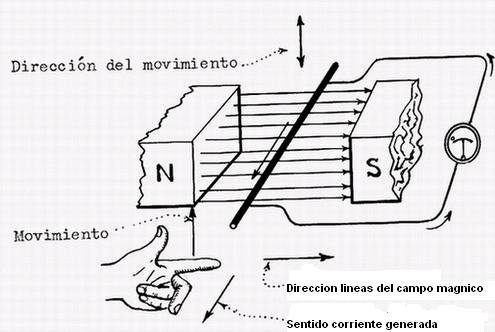
\includegraphics[scale=0.7]{dinamo.png}
    \caption{Dirección del campo magnético.}
  \label{fig1}
\end{figure}
\noindent
Este descubrimiento fue lo que dio lugar a los generadores eléctricos electromagnéticos (dinamos y alternadores).
\begin{figure}[H]
  \centering
  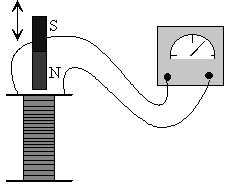
\includegraphics[scale=0.7]{bobina.png}
    \caption{Generación de energía eléctrica}
  \label{fig2}
\end{figure}
\noindent
Partiendo del primer caso, si en lugar de un conductor se coloca un espira girando dentro del campo magnético, en lugar de un conductor ahora se tienen dos conductores en forma de espira cortando el campo magnético. Por un lado de la espira la corriente que se genera es en un sentido y en el otro lado es en el sentido contrario es decir se generara una corriente eléctrica que se mueve alrededor de la espira. Cuando un lado de la espira está justo en el medio del campo magnético, el conductor no corta líneas de campo, y esto hace que en ese punto no se genere corriente. La gráfica de una vuelta completa de la espira generaría la siguiente señal eléctrica:
\begin{figure}[H]
  \centering
  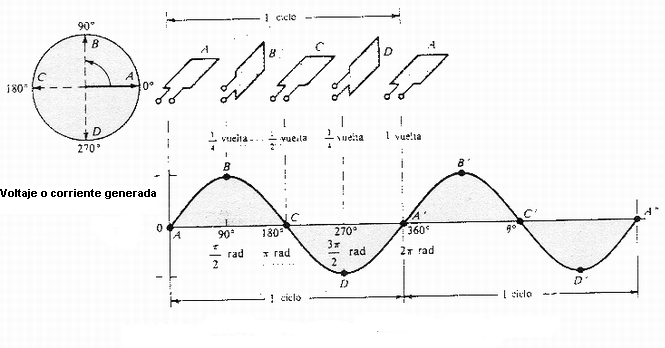
\includegraphics[scale=0.7]{image.png}
    \caption{Variación de la vuelta completa de una espira.}
  \label{fig3}
\end{figure}
\noindent
Como se puede observar se genera una onda de corriente alterna, cambia el sentido de la corriente y además la intensidad es variable. Si se unen los extremos de la espira a un receptor se tendrá un generador de corriente eléctrica, en este caso de corriente alterna (alternador).

\section{Generador síncrono}
\noindent
Se aplica una corriente se aplica corriente DC al devanado del rotor, la cual produce un campo magnético, entonces el rotor del generador gira mediante un motor primario y produce un campo magnético rotacional dentro de la máquina.\\
El generador síncrono está compuesto principalmente de una parte móvil o \textbf{rotor} y de una parte fija o \textbf{estator}.

\subsection*{Rotor}
\noindent
También conocido como inductor, pues es la parte que induce el voltaje en el estator. El núcleo del rotor es construido de lámina troquelada de acero al silicio, material de excelentes características magnéticas, con la finalidad de evitar pérdidas por histéresis y corrientes parásitas.\\
El yugo es una pieza continua con zapata polar, para así eliminar la dispersión del flujo por falsos contactos magnéticos. En la zapata polar se hacen barrenos para alojar el devanado amortiguador en jaula de ardilla, diseñado con el objeto de reducir armónicas en la forma de onda que entrega el generador.

\subsection{Alternador}
\noindent
Un alternador es una máquina eléctrica, capaz de transformar energía mecánica en energía eléctrica, generando una corriente alterna mediante inducción electromagnética.\\
Los alternadores están fundados en el principio de que en un conductor sometido a un campo magnético variable se crea una tensión eléctrica inducida cuya polaridad depende del sentido del campo y el valor del flujo que lo atraviesa.\\
Un alternador es un generador de corriente alterna que funciona cambiando constantemente la polaridad para que haya movimiento y genere energía.
\begin{figure}[H]
  \centering
  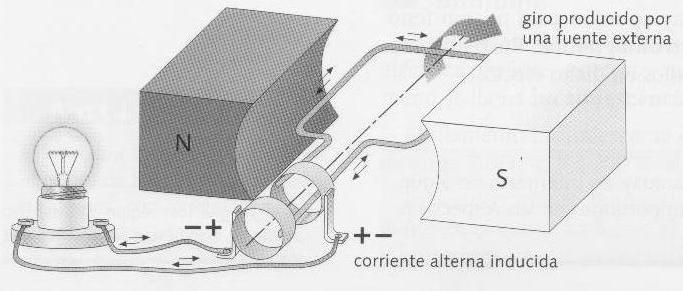
\includegraphics[scale=0.5]{alternador1.png}
    \caption{Diagrama simplificado de un alternador.}
  \label{fig4}
\end{figure}
\begin{figure}[H]
  \centering
  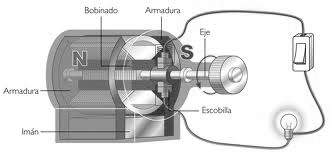
\includegraphics[scale=1]{alternador2.png}
    \caption{Alternador.}
  \label{fig5}
\end{figure}

\begin{figure}
 \includegraphics[]{×}
\end{figure}


\bibliographystyle{ieeetran}
\begin{thebibliography}{99}

\bibitem{chapman} Chapman, Stephen J. ``Electric Machinery Fundaentals''. Fourth EDITION, McGraw-Hill, 2005.

\bibitem{page1} Pagina \url{http://electricidad.usal.es/Principal/Circuitos/Descargas/DefinicionAlternador.pdf}

\bibitem{page2} Pagina \url{http://www.izt.uam.mx/newpage/contactos/anterior/n65ne/generador.pdf}

\end{thebibliography}
\end{document}